\section{Other Common DWS Architectures}
\label{sec:otherArchitectures}
After having introduced the reference architecture, this chapter aims to show other approaches for building Data-Warehouse-Systems. The main object of consideration is the distributed DWS architecture. It was invented by Ralph Kimball and can be seen as the counterpart to Inmon's hub and spoke architecture.\newline
Afterwards the characteristics of different data mart arrangements will be discussed. This information will be used later to deal with a flexible data provision.\newline
In the end, an outlook on different options regarding the data persistence in different layers will be given. This topic will get relevant when talking about the deployment of Data-Warehouse-Systems as collection of microservices by using the self-contained systems approach.

\subsection{Distributed Data Warehousing Architecture}
After having explained the reference architecture from A. Bauer, which implements the hub and spoke idea from Inmon, one very common alternative is presented. Ralph Kimball is another pioneer in this area who came up with a distributed data warehousing architecture based on data marts connected to a bus system \cite{surveyDWSArchs}. Figure \ref{fig:distributedWarehouseArchitecture} visualises this in more detail.
\begin{figure}[htb]
    \centering
    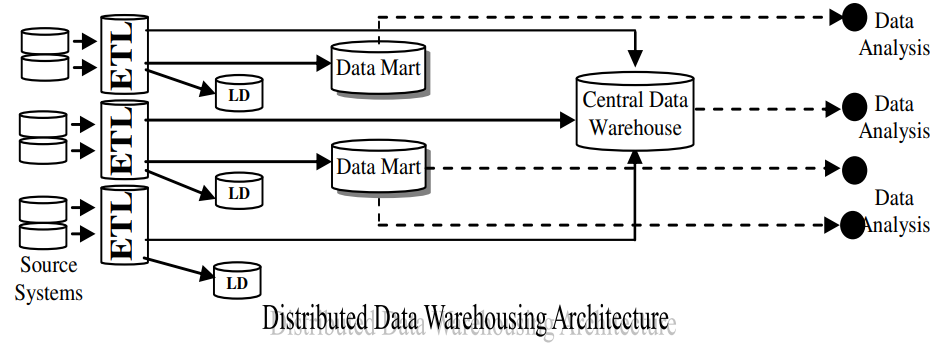
\includegraphics[scale=0.5]{pictures/DistributedDataWarehouseArchitecture.PNG}
    \caption{Distributed Data Warehousing Architecture by Ralph Kimball \cite{surveyDWSArchs}}
    \label{fig:distributedWarehouseArchitecture}
\end{figure}
\\In contrast to Inmon's approach, Kimball allows ''Everyone [...] to fabricate their database according to their requirements and department structures. All theixre independent repositories can be integrated as and when. [...]'' \cite{surveyDWSArchs}. Due to that the Central / core data warehouse results from those individual data mart and doesn't provide any consistency. This technique is also known as bottom-up approach for developing data warehouse Systems. Since the bus system is needed to ensure the interoperability between multiple data marts and the core data warehouse consistent data standards are therefore needed. Due to that, the design aspects are quite tough and the complexity is high. \cite{KimbalVSInmon}\newline
As Breslin states, ''Kimball's approach is a departure from traditional database development'' \cite[p.~19]{KimbalVSInmon} and therefore targets the IT professional himself.\newline

\subsection{Architectural Classification According to the Arrangement of Data Marts}
Next to the radical redesign of the hub and spoke architecture by Kimball's distributed data warehousing architecture, some alternatives regarding the organisation of data marts will be shown.\newline
\\
A central data warehouse consists of a single central instance with only one data mart which is used for all the analysis. This can be beneficial when a company-wide overview is needed. On the downside, it is only possible to apply one data model to this data mart. For department-specific analysis this could result in a huge problem. \newline
Instead, a distributed data warehouse consists of multiple data marts which are specific to the department. Each of this additional data storages has a separate schema. Hence, the creation of a new one results in more work. One problem is the company-wide perspective, which will get lost. \newline
A possible combination of the advantages from the two architectures above can be found in a central data warehouse with multiple distributed data marts. By applying this concept, it is possible to run company-wide analysis on the central data warehouse and to use data marts for the individual needs coming from various departments.
\newline
A last aspect which needs to be pointed out is the design aspects of dependent and independent data marts. Therefore, let us first have a look at dependent ones. Those are built upon the core data warehouse and might contain additional or aggregated information. Nevertheless, the underlying \acrshort{cdw} ensures a consistency of the information distributed to the data marts. An independent data mart won't have such layer beneath. Due to that, the information inside might be duplicated and distinct to a certain degree. An advantage of using an independent architecture is the simplicity of creating these. \cite{scriptRasch} \newline
\\
This section should have shown the various design possibilities of data marts inside a corporate data warehouse System. By thinking about a modern adaption of DWS architectures, it is necessary to construct new data marts easily without losing the company-wide point of view and still enable departments to come up with their own requirements for analysis. 

\subsection{Options Regarding the Persistent Data Handling}
After having introduced various structural options above, let us face the topic of data persistence in current data warehouse Systems.
All layers inside the DWS can be created with virtual data or with their own data persistence. For instance, it is possible to have a complete virtual DWS. \cite{sinz}\newline
\\
For now, let us start off with the ETL layer. It is quite common to have persistence inside the staging area which is used as temporal data storage. Especially during the data transformation, this can be quite beneficial. Besides, it is possible to use an \acrfull{ods} which was introduced by Inmon as ''an operational data store is a subject-oriented, integrated, volatile, current-valued, detailed-only collection of data in support of an organisations need for up-to-the-second, operational, integrated, collective information'' \cite{buildingTheDWS} This storage uses the result of the data transformation and integration to publish it in such an ODS to have real-time-data available in the DWS.\newline
In concern of data historicisation, the persistence can be contained in the supply area (e.g. data marts) or the CDW, which can be seen as a component for historising the data. Depending on the technologies which are used (e.g. \acrshort{olap} or \acrshort{rolap}), there are multiple recommendations which get elaborated in Sinz's article on the architecture for data warehouse Systems.
\begin{itemize}
    \item If a relational (\acrshort{sql}) interface is used it is sufficient to persist the data in the core data warehouse.
    \item While using multidimensional OLAP tools, it is common to store the information inside the supply area of the DWS.
    \item When using relational OLAP, it is common to have a relational persistence inside the data marts. It is not necessary to use a redundant data storage underneath but it is recommended due to a decoupling of the loading process. 
\end{itemize}
\cite{sinz}
\\
\\
After the most commonly used architectures for data warehouse Systems have been outlined and the requirements regarding a DWS have been pointed out, newer technologies are introduced. In detail, the fundamental ideas of microservice and event-based architectures as well as Business Process Management will be elaborated. Further on these technologies will align in order to result in the final draft of the presented architecture.